\documentclass{article}
\usepackage{../fasy-hw}
\usepackage{ wasysym }
\usepackage[pdftex]{graphicx}


\newcommand{\N}{\mathbb{N}}
%% UPDATE these variables:
\renewcommand{\hwnum}{2}
\graphicspath{ {./images/} }
\author{Peter Gifford, Ren Wall, Kyle Brekke, Madison Hanson Group: 7}
\collab{~}
\date{due: 20 September 2019}

\begin{document}

\nextprob
Give a linear-time algorithm that takes two sorted arrays of real numbers as
input, and returns a merged list of sorted numbers.  You should give your answer
in pseudocode.    Your answer should contain:
\begin{itemize}
    \item A prose explanation of the algorithm.
    
     This algorithm works by keeping a pointer on one item in each list. Using these pointers we can check how a number in one list compares to a spot in the other list. If the numbers are the same then they can be added both to the list and increment both pointers, if one is smaller than the other then we can add that to the list and increment that pointer. This way the pointers walk through the lists only having to check each item one time and putting them into a new list that is still sorted.
     
    \item Psuedocode. (Be sure to review the two resources on pseudocode that were
        posted as readings for Week 2!  I also suggest the algorithm /
        algorithmx package in LaTex.)
        
        See Below
        
         \begin{algorithm}
        \caption{Merged list of sorted numbers from two sorted lists}\label{sorted list}
        \begin{algorithmic}[1]
        \Procedure{Merge}{$A,B$}\Comment{A and B are sorted lists this sorts them into list c}
        		\State \textbf{in:}  Sorted lists A,B
		\State \textbf{out:}  Sorted list c, the combination of A and B
        		\State $c\gets list;$
		\State $i, j\gets 0;$
		\While{$i < A.size()  \&\&  j < B.size()$}
			\If{$A.get(i) == B.get(j)$}
				\State c.add(A.get(i), B.get(j));
				\State i++;
				\State j++;
			\ElsIf{$A.get(i) < B.get(j)$}
				\State c.add(A.get(i));
				\State i++;
			\ElsIf{$A.get(i) > B.get(j)$}
				\State c.add(B.get(j))
				\State j++;
			\EndIf
		\EndWhile
		\If{$i == A.size()$}
			\While{$j < B.size()$}
				\State c.add(B.get(j));
				\State j++;
			\EndWhile
		\EndIf
		\If{$j == B.size()$}
			\While{$i < A.size()$}
				\State c.add(A.get(i));
				\State i++;
			\EndWhile
		\EndIf
		\State return c;
	\EndProcedure
	\end{algorithmic}
	\end{algorithm}
        
    \item The decrementing function for any loop or recursion.
    
	 Let $\mathbb{X}$ denote the state space of the algorithm. We define the function $D \colon \mathbb{X} \to \N \cup \{0\}$ by $D( \mathbb{X}) = ( length(A) + length(B) )-(i + j)\newline $
    
    Each time through the loop either $i,j$ or both are incremented. The are in $\N$ and therefore eventually $i + j$ must eventually equal $ length(A) + length(B) $ and therefore break the loop.

    Let $\mathbb{X}$ denote the state space of the algorithm. We define the function $D \colon \mathbb{X} \to \N \cup \{0\}$ by $D( \mathbb{X}) =  length(A) - i\newline $

    Let $\mathbb{X}$ denote the state space of the algorithm. We define the function $D \colon \mathbb{X} \to \N \cup \{0\}$ by $D( \mathbb{X}) =  length(B) - j\newline$
    
    For the two loops above on each iteration, either i or j will be incremented and will eventually hit the same length as the list they are being subtracted from and therefore hit zero and break the loop.
    
   

    
    \item Justification of why the runtime is linear.
    
        The algorithm will go through every item in the lists exactly once since the counters i and j will increment until they hit the array size and therefore no item in the lists will have more than O(1) spent on it. All the loops run in O(n) and are not nested with all steps in between taking O(1). This mean that O(A.size()+B.size()) is the complexity and therefore it is run in linear time. 
    
\end{itemize}

\nextprob
EPI 15.4 (Generate the Power Set) gives code to compute the power set of a set
(without duplicates).  Present this problem and solution in your own words using
pseudocode.

This algorithm is aimed at getting all the possible sets that can be made from a given set. The solution below uses a form of recursion to repeatedly add and remove elements from the recursion branch so that it can reach the bottom and generate a new set.

  	\begin{algorithm}
	\caption{Power Sets}\label{power sets}
        \begin{algorithmic}[1]
		 \Procedure{generatePowerSets}{$inputSet$}\Comment{Startup function}
		 \State \textbf{in:} List of integers that is a the inputSet
		 \State \textbf{out: } List of Lists of Integers that are the power sets;  
		 \State powerSet $\gets$ list;
		 \State newList $\gets$ list;
		 \State directedPowerSet(inputSet, 0, newList, powerSet);
		 \State return powerSet;
		 \EndProcedure
		 
		 \Procedure{directedPowerSet}{$inputSet, toBeSelected, selectedSoFar, powerSet$}
		 	\State \textbf{in:} inputSet : the original input set, toBeSelected : the spot in inputSet that the algorithm is checking, selectedSoFar : list of spots in inputSet already checked, powerSet : list of power sets already selected
			\State \textbf{out: } None
		 	\If{$toBeSelected == inputSet.size()$}
				\State powerSet.add(selectedSoFar.asList());\Comment{Adds all of selected so far because they represent a powerSet to powerSet and ends because there is nothing left to check}
				\State return;
			\EndIf
			\State selectedSoFar.add(inputSet.get(toBeSelected)); 
			\State directedPowerSet(inputSet, toBeSelected + 1, selectedSoFar, powerSet);
			\State selectedSoFar.remove(selectedSoFar.size() - 1);
			\State directedPowerSet(inputSet, toBeSelected + 1, selectedSoFar, powerSet);
		 \EndProcedure
	\end{algorithmic}
	\end{algorithm}


\nextprob
In EPI 15.1 (The Towers of Hanoi Problem), prove that the algorithm as presented
terminates.  In particular, you should give the decrementing function for the
recursion.

\nextprob
For the stock market problem discussed in class on September 6th (and in CLRS
4.1), walk through
the algorithm for the following input:
$$\mathtt{price} = \{ 3, 6, 8, 2, 1, 10, 5, 7 \}. $$

This algorithm has the goal of taking a list of integers and finding the greatest gap between two numbers where the first number precedes the larger number in the list. We have displayed how this works by showing the inputs to the functions in the book at each step. The input is displayed as $n=array, n[position]:number_at_position$.
The entire list is put into the first function.
BuySell(\{n[1]:3, n[2]:6, n[3]:8, n[4]:2\{n[5]:1, n[6]:10, n[7]:5, n[8]:7\})\newline

The method call above splits the list in half and because the list is longer than two items it calls the BuySell function again with the two halves of the list.\newline
BuySell(\{n[1]:3, n[2]:6, n[3]:8, n[4]:2\}), BuySell(\{n[5]:1, n[6]:10, n[7]:5, n[8]:7\})\newline

The lists have been split in half again and once again get passed into BuySell. This step returns those sets up to the last recursion level to be used by compare in the next step\newline
BuySell(\{n[1]:3,n[2]: 6\}) BuySell(\{n[3]:8, n[4]:2\}), BuySell(\{n[5]:1, n[6]:10\}), BuySell(\{n[7]:5, n[8]:7\})\newline
return = \{n[1]:3,n[2]: 6\}\{n[3]:8, n[4]:2\}\{n[5]:1, n[6]:10\}\{n[7]:5, n[8]:7\}

Now that the lists are of size 2 or less, the compare function is called on two of the lists as well as the first element of the first list and second element of the second list and returns set of farthest points. \newline
compare(\{n[1]:3,n[2]:6\},\{n[3]:2,n[4]:8\},\{n[1]:3,n[4]:8\}) = \{n[3]:2,n[4]:8\}, compare(\{n[5]:1,n[6]:10\},\{n[7]:5, n[8]:7\},\{n[5]:1,n[8]:7\}) = \{n[5]:1, n[6]:10\}\newline
return = \{n[3]:2,n[4]:8\}\{n[5]:1,n[6]:10\}\newline

The same process as the last step is repeated with the new lists generated from the last step.\newline
compare(\{n[3]:2,n[4]:8\},\{n[5]:1,n[6]:10\},\{n[3]:2,n[6]:10\}) = \{n[5]:1,n[6]:10\}\newline

There was only one call of compare and therefore only one set is returned and this set is the answer.\newline
result = \{n[5],n[6]\}

\nextprob
Prove using induction that the closed form of:
$$T(n) = \begin{cases}
            1        & n=1\\
            T(n-1)+n & n>1
         \end{cases}
$$
is $O(n^2)$.

Proof by induction:\\
Base Case: $T(1) = 1$ takes $1$ step.\\
Inductive assumption: $T(n-1)$ takes $m$ steps.\\
Inductive Step: $T(n)$ takes one more step than $t(n-1)$ so $T(n)$ takes $m + 1$ steps.\\
By induction we can see that $m + 1 = n$ so $T(n)$ takes $n$ steps. $T(n) \in O(n) \subset O(n^2 )$

\nextprob
What is the closed form of the following recurrence relations?  Use Master's
theorem to justify your answers:
\begin{enumerate}
    \item $T(n) = 16 T(n/4) + \Theta(n)$
    
    $a = 16, b = 4, n^2, f(n) = n, case  1\newline$
    $\epsilon = 1$
    T(n) =  $\Theta(n^2)$
    
    \item $T(n) = 2 T(n/2) + n \log{n}$
    
    $a = 2, b = 2, n^1, f(n) = n\log{n}, case 3\newline$
    $f(n) = \Theta(n^c), c = 2\newline$
    $\log_{2}2 < 2$ satisfies condition for case 3 \newline
    T(n) = $\Theta(n\log{n})$
    
    \item $T(n) = 6 T(n/3) + n^2 \log{n}$
    
   $a = 6, b = 3, n^1.6, f(n) = n^2, case 3\newline$
   $f(n) = \Theta(n^c), c = 2\newline$
    $\log_{3}6 < 2$ satisfies condition for case 3 \newline
    T(n) = $\Theta(n^2)$
    
    \item $T(n) = 4 T(n/2) + n^2$
    
    $a = 4, b = 2, n^2, f(n) = n^2, case 2 \newline$
    T(n) = $\Theta(n^2\log{n})$
    
    \item $T(n) = 9 T(n/3) + n$
    
    $a = 9, b = 3, n^2, f(n) = n, case 1\newline$
    $\epsilon = 1$
    T(n) = $\Theta(n^2)$
    
    
\end{enumerate}
Note: we assume that $T(1)=\Theta(1)$ whenever it is not explicitly given.

\nextprob
\emph{The skyline problem:} You are waiting for the ferry across the river to
get into a big city, and notice
$n$ buildings in front of you.  You take a photo, and notice that each building
has the silhouette of a rectangle.  Suppose you  represent each building as a
triple $(x_1,x_2,y)$, where the building can be seen from $x_1$ to $x_2$
horizontally and has a height of $y$.  Let $\mathtt{rect(b)}$ be the set of
points inside this rectangle (including the boundary).  Let $\mathtt{building}$ be the set of $n$
triples. Design an algorithm that takes $\mathtt{buildings}$ as input, and
returns the skyline, where the skyline is a sequence of $(x,y)$ coordinates
defining $\cup_{b \in \mathtt{buildings}} \mathtt{rect}(b)$.

Goal is to use a divide and conquer algorithm (said in class).

This algorithm takes in the coordinate of a rectangular buildings as {x1,y,x2}. With these, the outline of the "skyline" they generate is returned using a divide and conquer strategy similar to merge sort. However instead of sorting numbers this returns the better point to be represented on the skyline.

  	\begin{algorithm}
	\caption{Skyline Problem}\label{skyline}
        \begin{algorithmic}[1]
		 \Procedure{getSkyline}{$buildingCoord$}
		 \State \textbf{in: } list of skyline variables as buildingCoord.
		 \State \textbf{out: } final list of coord for the skyline.
		 \State return calculateSkyline(buildingCoord, 0, buildingCoord.size() - 1)	
		 \EndProcedure
		 
		 \Procedure{calculateSkyline}{$arr, l, h$}
		 \State \textbf{in: } list of coordinate as arr, the low spot in the array as l, the high spot in the array as h
		 \State \textbf{out: } list of coordinate for the skyline
		 
		 \If{$ l == h $}\Comment{what method returns once there is no more options to split}
		 \State $res \gets list;$
		 \State res.add(arr[0],arr[1]);
		 \State res.add(arr[2],0);
		 \State return res;
		 \EndIf
		 
		 \State $mid\gets (l + h)/2$\Comment{Splitting down the middle like merge sort}
		 
		 \State $listLeft \gets calculateSkyline(arr, l, mid);$
		 \State $listRight \gets calculateSkyline(arr, mid + 1, h);$
		 \State $toReturn \gets mergeSkylines(listLeft, listRight)$
		 \State return toReturn;
		 
		 \EndProcedure
		 
		 \Procedure{mergeSkylines}{$left, right$}
		  \State \textbf{in: } lists of coordinate needed to be merged as left, right
		 \State \textbf{out: } merged and 'sorted' lists of the resulting skyline
		 \State $toReturn \gets list$
		 \State $i, j \gets 0$
		 \State $heightLeft, heightRight \gets 0$
		\While{$i < left.size() \&\& j < right.size()$}
		\If{$left[i][0] < right[j][0]$}
		\State $x \gets left[i][0];$
		\State $heightLeft \gets left[i][2];$
		\State $maxHeight \gets max(heightLeft, heightRight);$\Comment{max gets the maximum value of values entered since only the tallest building can be seen}
		\State toReturn.add((x, maxHeight));
		\State $i \gets i + 1;$
		\Else
		\State $x \gets right[i][0];$
		\State $heightRight \gets right[i][2];$
		\State $maxHeight \gets max(heightLeft, heightRight);$
		\State toReturn.add((x, maxHeight));
		\State $j \gets j + 1;$
		\EndIf
		\EndWhile
		\While{$i < left.size()$}\Comment{If one list is bigger than the other we need to add all the rest of the skylines because we can see all of them.}
		\State $toReturn \gets left[i];$
		\State $i \gets i + 1;$
		\EndWhile
		\While{$j < right.size()$}
		\State $toReturn \gets right[i];$
		\State $j \gets j + 1;$
		\EndWhile
		\State return toReturn;
		\EndProcedure
		 
	\end{algorithmic}
	\end{algorithm}

\nextprob
The \texttt{rand()} function in the standard C library returns a
uniformly random number in \texttt{[0,RANDMAX-1]}. Does \texttt{rand}()$\mod n$
generate a number uniformly distributed in $[0,n-1]$?

Note I: This is the second variant in EPI 5.12.

Note II: When asked questions of this form, you are expected to justify your
answer.

When you take \texttt{rand}()$\mod n$ it does  generate a number uniformly distributed in $[0,n-1]$. This is because the \texttt{rand()} function generates uniformly distributed random numbers, so the numbers generated by \texttt{rand}()$\mod n$ will be a uniform distribution of numbers with the numeric possibilities of (RANDMAX-1)/(n). This new random distribution would be a uniform distribution in $[0,n-1]$, meaning \texttt{rand}()$\mod n$ does  generate a number uniformly distributed in $[0,n-1]$.


\nextprob

Algorithms where we use randomization to find a deterministic answer are known
as Las Vegas algorithms.  Monte Carlo algorithms also use randomization, but
might not always give the right answer; however, they either have a high
probability of being correct or close to correct.

\begin{enumerate}[(a)]
    \item Give a Monte Carol algorithm to estimate~$\pi$.
    
    (algorithm taken from http://www.eveandersson.com/pi/monte-carlo-circle)
    
    Have a circle of radius R inside a square of 2R by 2R.
    
    Generate n numbers randomly.
    
    The numbers that are inside of the circle are M.
    
    \[ pi = \frac{4*M}{N} \]
    
    \item Let $n$ be the number of random numbers used by your algorithm.
        Explain why as $n \to \infty$, the expectation of the output for your
        algorithm is~$\pi$.
        
    Proof: 
    
    As $n \to \infty $, the expectation of our output is $\pi$.
    
    Since the area of the square of size 2R by 2R divided by the area of the circle equals to pi/4 the amount of random points that fall in the circle divided by the amount of random points that are generated will be equivalent to that same circle and square ratio, which then divided by four calculates $\pi$.
    
    Thus as $n \to \infty $, the expectation of our output is $\pi$, which was to be shown.
    
    \item Implement this algorithm and plot a line graph of
        the values returned for at least $10$ values of~$n$. Code for implementation in Appendix A.

        
       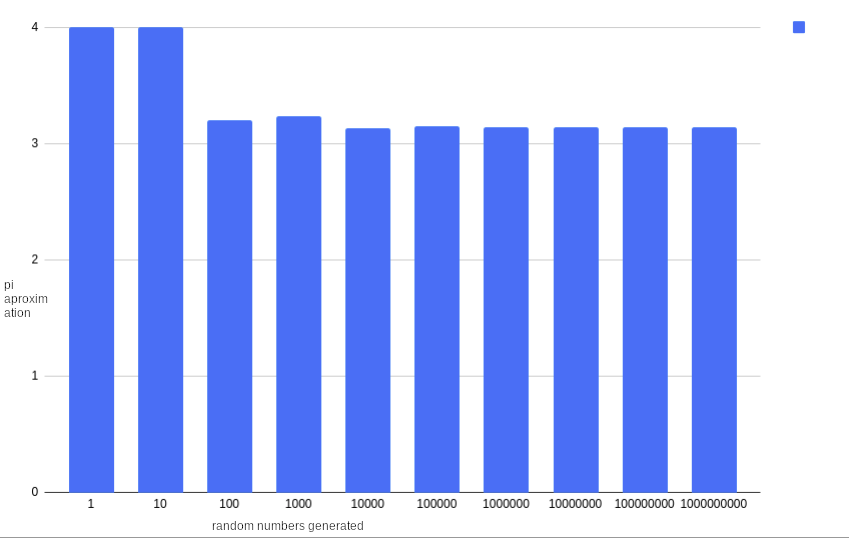
\includegraphics[scale=1]{images/graph.png}
        
        
        
        
\end{enumerate}

Note: We can use the function \texttt{randReal}$(a,b)$ that returns a random
real number between $a$ and $b$ inclusive.

\nextprob
Appendix A Code for implementation of Monte Carlo Method:

import java.util.Random;

public class CarloMonteAndHisPython\{

\quad     public static void main(String []args)\{

\quad \quad        double circleArea = 12.5663706144;

\quad \quad        double squareArea = 16.0;

\quad \quad        double random =0.0;

\quad \quad        double pi = 0.0;

\quad \quad        int inCircle = 0;

\quad \quad        int inSquare = 0;

\quad \quad        int n = 0;

\quad \quad        Random randomizer = new Random();
        
\quad \quad        for(int i = 0; i <1000;i++)\{

\quad \quad \quad            random =randomizer.nextDouble()*16.0;

\quad \quad \quad             if(random > circleArea)\{

\quad \quad \quad \quad                 inSquare = inSquare + 1;

\quad \quad \quad             \}else if(random <= circleArea)\{

\quad \quad \quad \quad                 inSquare = inSquare + 1;

\quad \quad \quad \quad                 inCircle = inCircle + 1;

\quad \quad \quad             \}

\quad \quad \quad             n=i;
\quad \quad        \}
\quad \quad  
\quad \quad          n=n+1;

\quad \quad          pi = (4.0*(inCircle))/(inSquare);

        
        
\quad \quad          System.out.println("Pi using the Monte Carlo method with "+n+" digits is "+pi);
        
     \}

\}

\end{document}
